% ===== PDF p.041 (原书 p.33) =====
% 原书本章节号用阿拉伯数字（1 はじめに、2 正多面体の分類…），故在此改为阿拉伯数字；章末 reflist 之后恢复罗马数字
\renewcommand{\thesection}{\arabic{section}}
\chapter{正多面体与镜像对称}
\chapterauthor{高橋篤史}{[大阪大学大学院理学研究科]}

\section{引言}

本章想谈一谈正多面体与奇点之间的关联。为此，先来思考下面这个问题：

\begin{problem}{1}
  求满足不等式
  \begin{equation}
    \frac{1}{p}+\frac{1}{q}+\frac{1}{r}>1 \tag{1}
  \end{equation}
  的全部正整数三元组 $(p,q,r)$。
\end{problem}

这个问题的答案可以简洁地写成
\begin{equation}
  (p,q,r)=
  \begin{cases}
    (m,\,l-m+1,\,1), & 1\le m\le l,\\
    (l-2,\,2,\,2), & 4\le l,\\
    (3,3,2),\ (4,3,2),\ (5,3,2),
  \end{cases}
  \tag{2}
\end{equation}
不过，正是这个简单的事实，支配着许多深刻的数学现象\footnote{ADE 分类型定理的证明，都要经由与各自主题相关的不变量，归结为解这个不等式。}。
% [Tutor Note: 问题 1 的正整数解分成无穷族 $(m,l-m+1,1)$ 与有限个例外 $(3,3,2)$、$(4,3,2)$、$(5,3,2)$；后三个正是正四面体、正八面体、正二十面体对应的三元组。它与 ADE 型单奇点、$SO(3)$ 有限子群、Dynkin 图 $A$--$D$--$E$ 的分类是同一件事。]

正多面体的研究从 2000 多年前就开始了，正多面体与奇点的关系则从大约 100 年前开始被研究。另一方面，从本书的主题——与超弦理论相关联的最前沿理论——镜像对称的观点来看，它们也仍然是研究余地很充分的深刻对象。因此，从初等的内容到极其专业的内容都有，其中不少内容，即便是数学爱好者也能亲近、享受。所以，这里与第 5 章、第 11 章换一换气氛，从初等的话题开始
% ===== PDF p.042 (原书 p.34) =====
解说。

\section{正多面体的分类}

先来复习一下正多边形。

\begin{definition}{2}
  平面上闭的凸多边形，若它的各条边彼此全等、各个内角彼此相等，就称为正多边形。特别地，当边数为 $n$ 时，称为正 $n$ 边形。
\end{definition}

正 $n$ 边形有经过所有顶点的圆（外接圆）和与所有边相切的圆（内切圆）。这两个圆的圆心重合，我们把它叫作正 $n$ 边形的中心。正 $n$ 边形的内角是 $\left(1-\dfrac{2}{n}\right)\cdot 180^\circ$。通常我们认为“内角大于 $0^\circ$”，但把 $n=2$ 也包含进来考虑更自然，所以这里设 $n\ge 2$。

接下来给出正多面体的定义。

\begin{definition}{3}
  各面都是彼此全等的正多边形，且每个顶点周围聚集着相同数目的面，这样的三维空间内的闭凸多面体称为正多面体。特别地，当面数为 $n$ 时，称为正 $n$ 面体。
\end{definition}

我们来考察对怎样的 $n$ 存在正多面体。设各面是正 $p$ 边形，且每个顶点周围聚集 $q$ 个面。那么，由凸多面体的条件，聚集在某个顶点处的各正 $p$ 边形的内角之和必须满足
\begin{equation}
  \left(1-\frac{2}{p}\right)\cdot 180^\circ\cdot q<360^\circ \tag{3}
\end{equation}
把这个式子变形，就得到
\[
  \frac{1}{p}+\frac{1}{q}+\frac{1}{2}>1.
\]
因此，作为正多面体存在的必要条件，$(p,q)$ 的
% ===== PDF p.043 (原书 p.35) =====
组合只能是
\begin{equation}
  (p,q)=
  \begin{cases}
    (p,2),\ (2,q),\\
    (3,3),\ (3,4),\ (3,5),\ (4,3),\ (5,3),
  \end{cases}
  \tag{4}
\end{equation}
这一点就明白了。反过来，对每个 $(p,q)$ 的组合 $(3,3),(3,4),(3,5),(4,3),(5,3)$，分别对应正四面体、正八面体、正二十面体、立方体、正十二面体。另外，对组合 $(2,p,2)$ 及 $(2,2,q)$，约定考虑把 2 枚正 $p$ 边形粘合、以及把 $q$ 枚“正 2 边形”粘合所得的“塌缩的多面体”。这些对象乍看之下有些奇怪，但若与不等式（1）的解的分类对照，读者大概也会觉得把它们包含进来更自然。请注意：交换 $p$ 与 $q$ 的角色，就等于交换正多面体的顶点与面（的中心）的角色。这样的操作叫作取对偶多面体。下面考察的对象只限于在这个操作下不变的东西，所以以下设 $p\le q$。
% [Tutor Note: 所谓“塌缩的多面体”，就是二面体（dihedron）：把正 $p$ 边形的两面粘合，或把 $q$ 个“正 2 边形”沿边粘合。它的旋转对称群是二面体群，正好补上了后面 $SO(3)$ 有限子群分类中漏掉的那一族。]

正多边形有外接圆和内切圆。同样，正多面体有经过所有顶点的球（外接球）和经过所有面中心的球（内切球），这一点可以简单地证明\footnote{用坐标来描述正多面体就很容易看懂了。}。外接球与内切球的球心重合，我们把它叫作正多面体的中心。正多面体的所有面都全等，是“对称性”非常好的图形。下面用稍微数学化的方式把这一点表达出来。

\begin{definition}{4}
  即使各顶点、边、面的位置发生变化，正多面体整体仍与原来的正多面体重合，这样的操作称为正多面体的对称性。
\end{definition}

这里我们关注由空间的旋转引起的对称性（旋转对称性）。于是可以知道下面的事实。

\begin{itemize}
  \item 连续旋转 2 次，可以表示成 1 次旋转。
  \item 旋转 1 次后，再施加与它“相反”的旋转，就回到原状。
\end{itemize}

% ===== PDF p.044 (原书 p.36) =====
对此，我们再定一条规则：把“完全不旋转正多面体”也当作旋转对称性的一种来考虑。这样，它就成为一个叫作群的数学概念\footnote{这里省略了，不过积的合成律显然成立。}。群是为了从数学上理解“对称性”而引入的概念，这里得到的正多面体的旋转对称性，特别地叫作正多面体群。对称操作只由顶点、边、面的置换决定，所以正多面体群由有限个元素（对称性）组成，也就是有限群。

\section{正多面体群}

在上面的初等几何讨论中，我们把正多面体群作为三维欧几里得空间中全体旋转对称性所构成的群的一部分引入了。更准确地说，正多面体群是特殊正交群 $SO(3)$ 的有限子群。其实反过来关系也是已知的：$SO(3)$ 的有限子群只有循环群 $\Z/l\Z$ 和这些正多面体群。
% [Tutor Note: 原文如此。$SO(3)$ 有限子群的完全分类是：循环群 $C_l$、二面体群 $D_l$、正四面体群 $T$、正八面体群 $O$、正二十面体群 $I$。原文把二面体群归入了上一段所说的“塌缩的多面体”的正多面体群，对照（6）式中指数取 $(2,2,q)$ 的情形即可理解。]

我们来具体描述正多面体群。不妨想象地球的自转：给出一个空间旋转，与给出这个旋转的轴（以地球为例，就是连接北极与南极的地轴），是同一回事。给出正多面体旋转对称性的旋转轴，只要把外接球想成地球，考察哪些点可以成为北极或南极，就能求出来。可以看出只有下面 3 种可能：

\begin{itemize}
  \item 旋转轴是连接顶点与正多面体中心的直线。
  \item 旋转轴是连接边的中点与正多面体中心的直线。
  \item 旋转轴是连接面的中心与正多面体中心的直线。
\end{itemize}

下面用它来对正四面体的情形再稍微详细地考察旋转对称性。如图 1 所示，旋转轴有 2 种。我们把绕通过边中点与中心的旋转轴旋转 $180^\circ$ 的操作记作字母 $c$，把绕通过顶点的旋转轴旋转 $120^\circ$ 的操作记作字母 $b$\footnote{关于旋转的方向，这里省略了说明。请适当地补上，完成下面的讨论。}。另外，把旋转的组合像通常的乘法那样用积表示，把“不旋转”这件事（作为乘法单位元）用 $1$ 表示。于是，考察旋转轴与旋转角，就能容易地推出 $c^2=1=b^3$

% ===== PDF p.045 (原书 p.37) =====
\begin{figure}[htbp]
  \centering
  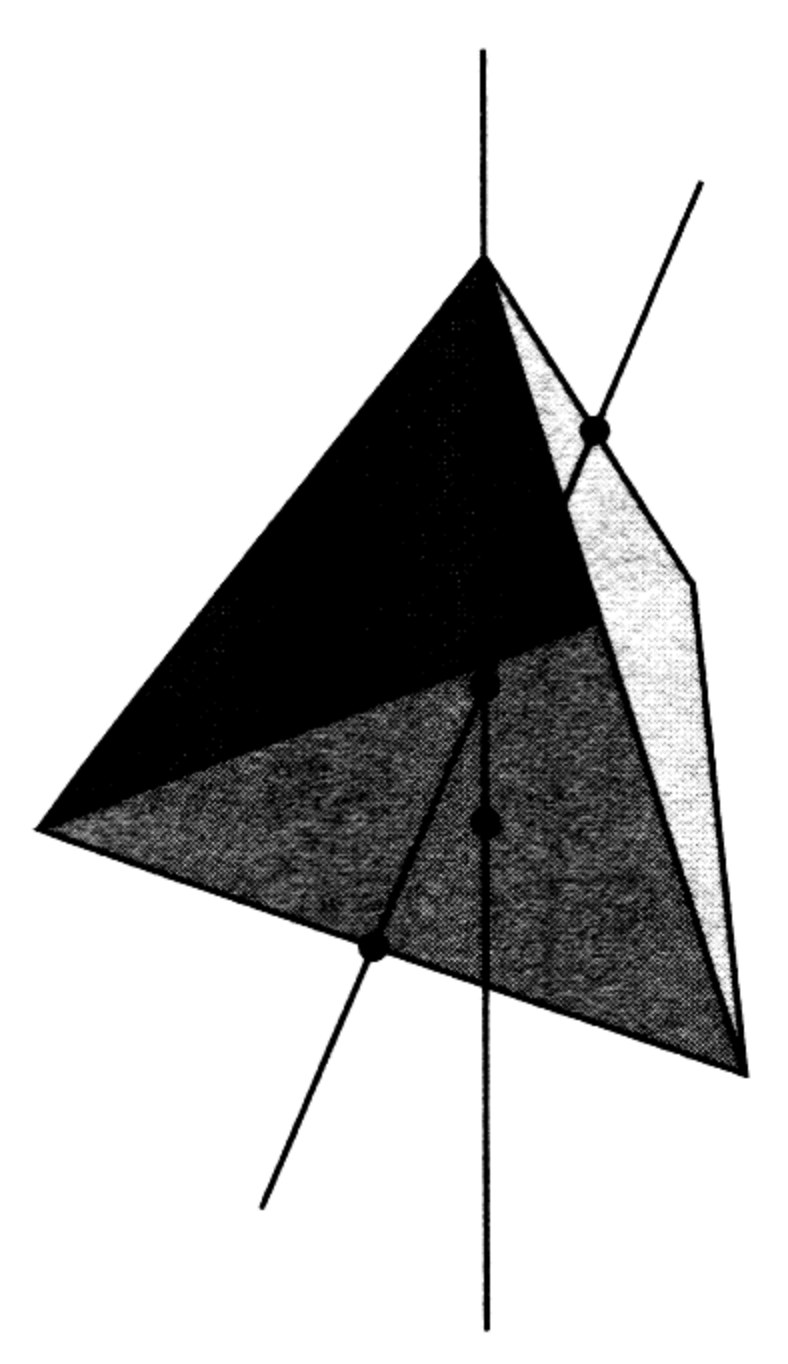
\includegraphics[width=0.35\linewidth]{figures/ch03-fig1.png}
  \figtitle{1}{正四面体的 2 种旋转轴（原书 p.37）}
\end{figure}%
% [Tutor Note: 图 1 中两类轴：过顶点与中心（对面中心）的轴，绕其旋转 $120^\circ$（对应 $b$）；过边中点与中心的轴，绕其旋转 $180^\circ$（对应 $c$）。正四面体的旋转对称群 $T$ 有 12 个元素，正是由这两种旋转生成的。]
以及 $(bc)^3=1$。令 $a:=(bc)^{-1}$，就得到从用生成元与关系式表达的群
\begin{equation}
  \langle a,b,c \mid a^3=b^3=c^2=abc=1\rangle \tag{5}
\end{equation}
到正多面体群的同态。进一步作几何上的考察，可以证明这给出的是同一个群（群同构）\footnote{很遗憾，这里没法展开。有兴趣的读者请努力把证明补上吧。}。
% [Tutor Note:（5）式即正四面体群 $T\cong A_4$ 的一组生成元与关系式。三个生成元对应三种旋转：$a$、$b$ 各为 $120^\circ$ 顶点旋转，$c$ 为 $180^\circ$ 边中点旋转；关系 $a^3=b^3=c^2=abc=1$ 的指数 $(3,3,2)$ 就是正四面体的 $(p,q,r)$。]

值得注意的是，在生成元 $a,b,c$ 的指数上，正多面体分类时出现过的组合 (3,3,2) 再次登场了。这并非偶然。实际上，与上面概述正四面体群时一样，由组合 $(p,q,2)$ 刻画的正多面体群具有
\begin{equation}
  \langle a,b,c \mid a^p=b^q=c^2=abc=1\rangle \tag{6}
\end{equation}
这样用生成元与关系式给出的表示。

% ===== PDF p.046 (原书 p.38) =====
\section{轨道空间}

正多面体群的任意元素都是旋转对称性，也就是特殊正交群 $SO(3)$ 的元素，因此特别地会把外接球映到外接球。于是，就可以考虑正多面体群作用于外接球所得到的轨道空间\footnote{本来想叫它轨形（orbifold），但为了与第 11 章“奇点与镜像对称”中的 Landau--Ginzburg 轨形模型相区别，这里改用了别的说法。}。这里所说的轨道空间，就是把群的元素互相移到的（外接球面上的）点视为同一点而得到的图形\footnote{要准确理解下面要讲的内容，需要比较高级的知识与理解。例如，作为通常的代数簇，轨道空间是 $\PP^1$（球面）；但若加上下面要说明的“尖点”所带的附加数据，作为代数叠来考察会更自然。}。它是一个“在 3 个特别点处变尖的球面”。

稍微具体地说明一下。由式 (6) 对正多面体群的描述可知，连结边中点与中心的旋转轴，它与外接球的交点被满足 $c^2=1$ 的元素 $c$ 固定。并且，旋转轴附近的点，对正多面体群的任何元素来说都映到别的点。也就是说，轨道空间中对应被元素 $c$ 固定的点的那个点，可以看成是“$1/2$ 点”：该点周围的角度总和不是 $360^\circ$，而是其一半 $180^\circ$ 的尖点。同样，对 $a,b$ 作考虑，就得到“$1/p$ 点”以及“$1/q$ 点”。

\section{轨道空间的代数描述}

下面稍作说明：带 3 个尖点的球面如何用代数几何来描述。把球面看作射影直线 $\PP^1=\C\cup\{\infty\}$ 时，其上任意的 3 点都能通过全纯自同构（分式线性变换）映到 $0,\infty,1$。因此，可以假定这 3 个尖点分别位于 $0,\infty,1$，并分别是“$1/p$ 点”“$1/q$ 点”“$1/r$ 点”。这时，这个轨道空间 $\PP^1_{p,q,r}$ 可以表示为
\begin{equation}
  X_{p,q,r} := \{\, Z_0^p - Z_1^q + Z_2^r = 0 \,\} \subset \C^3 \tag{7}
\end{equation}
\begin{equation}
  \PP^1_{p,q,r} \cong [X_{p,q,r}\setminus\{0\}/G_{p,q,r}] \tag{8}
\end{equation}
这样的形式\footnote{$G_{p,q,r}$ 是由 $\C^*:=\C\setminus\{0\}$ 对 $\Z/p\Z\times\Z/q\Z\times\Z/r\Z$ 作扩张得到的交换群；括号 $[\ ]$ 表示的不是代数簇意义下的商，而是商叠。}。要讲得严格，会涉及相当专门的内容，不过这里想尽量简单地说明上面式子的意义。

射影平面 $\PP^2:=\C^3\setminus\{0\}/\C^*$ 的一次超曲面
\[
  z_0-z_1+z_2=0,\qquad [z_0,z_1,z_2]\in\PP^2
\]
所表示的部分图形（部分流形）与射影直线 $\PP^1$ 同型。特别地，可以把 $z_0/z_1$ 看作 $\PP^1$ 的坐标。因此，令 $z_0:=Z_0^p$，
% ===== PDF p.047 (原书 p.39) =====
\begin{figure}[htbp]
  \centering
  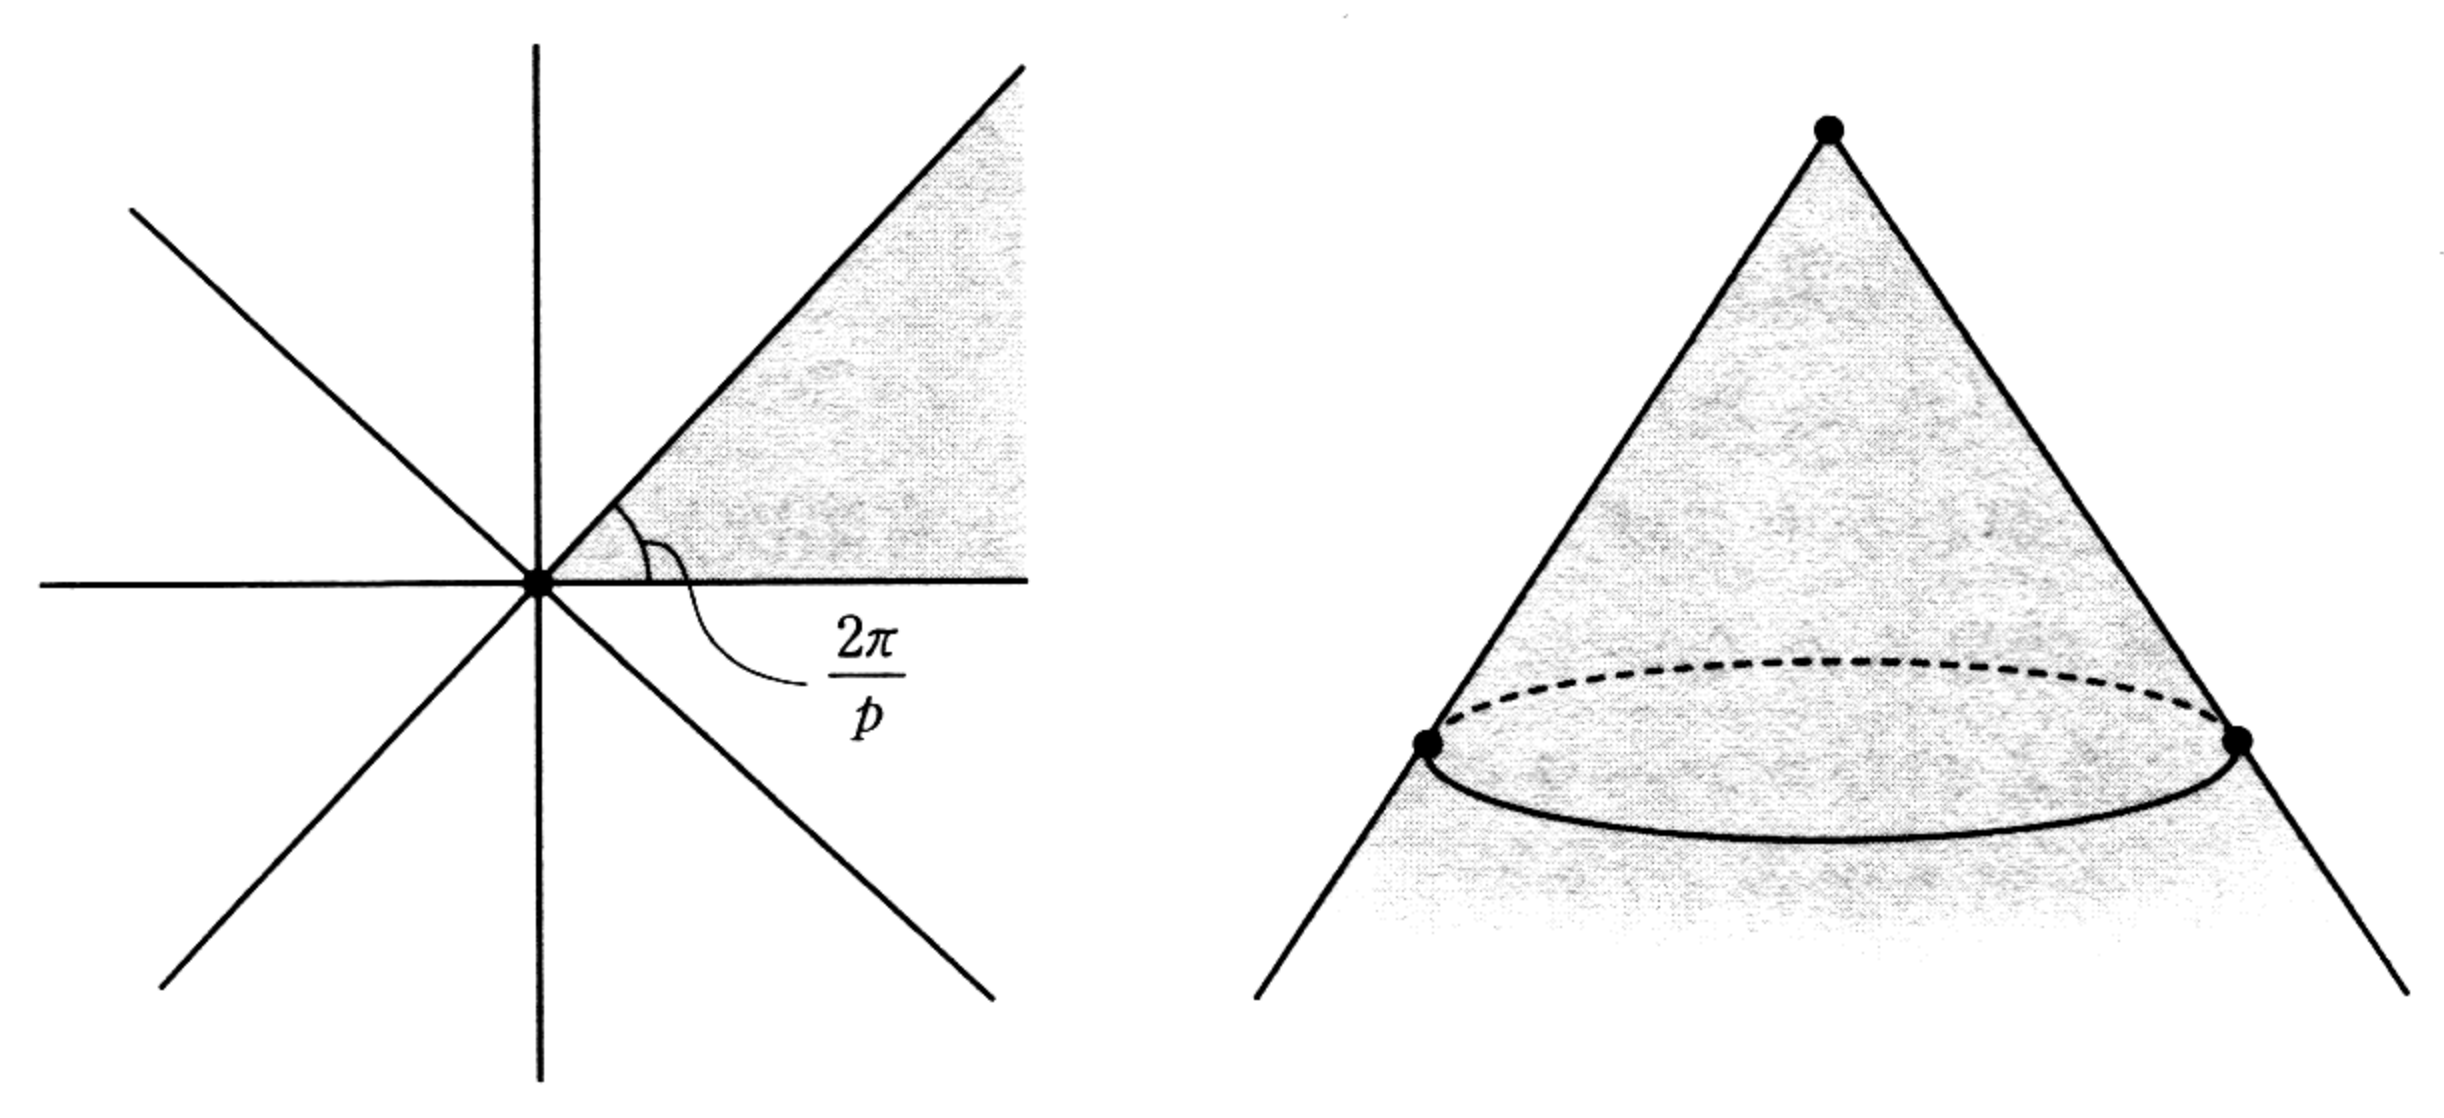
\includegraphics[width=0.9\linewidth]{figures/ch03-fig2.png}
  \figtitle{2}{满足 $a^p=1$ 的元素 $a$ 所固定的点周围的状况（原书 p.39）}
\end{figure}%
% [Tutor Note: 图 2 是“$1/p$ 点”的直观示意：左图中张角 $2\pi/p$ 的扇形把两条边粘合起来，就得到该尖点；右图中圆锥的顶点表示尖点，球面上被固定点的轨道被压成一个点。]
$z_1:=Z_1^q$，$z_2:=Z_2^r$，作这样的变量替换，就可以把 $\PP^1_{p,q,r}$ 看成 $\PP^1$\footnote{要使讨论准确，需要考察 $G_{p,q,r}$ 与 $\C^*$ 的对应，以及它们对多项式环的作用。}。进一步，点 $[Z_0,Z_1,Z_2]=[0,1,1]\in\PP^1_{p,q,r}$ 对应 $\PP^1$ 的原点，由 $x=X^p$ 这一变量替换的性质可知，它是“$1/p$ 点”。同样，点 $[1,0,-1]$、$[1,1,0]$ 分别是位于 $\infty\in\PP^1$ 的“$1/q$ 点”与位于 $1\in\PP^1$ 的“$1/r$ 点”。

希望读者能体会到：仅凭 $(p,q,r)$ 这一组信息，就能简单地描述轨道空间 $\PP^1_{p,q,r}$。

\section{孤立超曲面奇点与轨道空间}

那么，这里来讲一个乍看之下内容不同的话题。考虑 3 变量的（加权）齐次孤立超曲面奇点 $f(x_1,x_2,x_3)$\footnote{这也请参照第 11 章。}。

% ===== PDF p.048 (原书 p.40) =====
这时，变量 $x_1,x_2,x_3$ 与多项式 $f$ 分别具有次数 $a_1,a_2,a_3$ 与 $h$，由此可知 $\C^*$ 自然地作用在 $\C^3$ 以及 $f$ 的零点集合
\[
  X_f := \{\, f(x_1,x_2,x_3)=0 \,\} \subset \C^3
\]
上。由于 Jacobi 环在 $\C$ 上是有限维的，可以证明 $X_f\setminus\{0\}$ 没有奇点，所以由 $\C^*$ 得到的商空间 $C_f:=X_f\setminus\{0\}/\C^*$ 具有光滑紧黎曼面的结构。

不过，这种情形下也存在被（有限个）$\C^*$ 的元素固定的 $X_f$ 上的点。因此，与考虑正多面体群对球面的作用时一样，考虑轨道空间
\begin{equation}
  \mathcal{C}_f := [X_f\setminus\{0\}/\C^*] \tag{9}
\end{equation}
是自然的。请把这个轨道空间 $\mathcal{C}_f$ 理解为在黎曼面 $C_f$ 上附加了若干个尖点的信息。
% [Tutor Note: 原文用 $\mathcal{C}_f$ 记带尖点信息的轨道空间，即商叠 $[X_f\setminus\{0\}/\C^*]$；用 $C_f$ 记它的粗模空间，后者是光滑紧黎曼面。]

\section{不可思议的对应}

到此为止，我们引入了两种轨道空间 $\PP^1_{p,q,r}$ 与 $\mathcal{C}_f$。它们之间有极其密切的关系。实际上，下面的事实成立。

\begin{theorem}{5}
  对正整数的组 $(p,q,r)$，存在奇点 $f$ 与有限群 $G_f$，使得 $\PP^1_{p,q,r}$ 与 $[\mathcal{C}_f/G_f]$ 作为轨道空间同型\footnote{群 $G_f$ 依组 $(p,q,r)$ 代数地确定。在下面的例子中，$G_f$ 可以取为只由单位元组成的平凡群。}。
\end{theorem}

更精确地说，对于（分次）环 $\C[Z_0,Z_1,Z_2]/(Z_0^p-Z_1^q+Z_2^r)$，可以系统地构造出与 $\C[x,y,z]/(f)$ 同型的子环。

举一个具体的例子吧。设 $1/p+1/q+1/r>1$。这时 $f$ 可以按下页的表那样选取：

通过轨道空间，可以看到正多面体群与 D·E 型奇点之间有着不可思议的对应关系。
% ===== PDF p.049 (原书 p.41) =====
\begin{table}[htbp]
  \centering
  \begin{tabular}{ccc}
    \toprule
    $(p,q,r)$ & $f$ & 型\\
    \midrule
    $(m,\,l-m+1,\,1)$ & $x^{l+1}+yz$ & $A_l$\\
    $(l-2,\,2,\,2)$ & $x^{l-1}+xy^2+z^2$ & $D_l$\\
    $(3,3,2)$ & $x^4+y^3+z^2$ & $E_6$\\
    $(4,3,2)$ & $x^3+xy^3+z^2$ & $E_7$\\
    $(5,3,2)$ & $x^5+y^3+z^2$ & $E_8$\\
    \bottomrule
  \end{tabular}
\end{table}%
% 原书此表无表号、无表题，故不加 \tabtitle（reports/ch03.md 记一笔）。
这些奇点称为 ADE 型奇点，是最基本也最重要的一类奇点。

最初发现并研究它的，是 Klein。因此，ADE 型奇点有时也被叫作 Klein 奇点。

\section{与镜像对称的关联}

读到这里，读者大概觉得还完全看不到镜像对称。然而，定理 5 的背后隐藏着镜像对称。对整数的组 $(p,q,r)$，对应着奇点与有限群的组 $(f,G_f)$。这里与第 11 章的记号相反，但令 $\tilde G_f:=G_f\times\Z/h\Z$ 时，存在奇点 $f^*$，使 $(f,\tilde G_f)$ 与 $(f^*,\{1\})$ 构成拓扑镜像对。实际上，对奇点 $f^*$ 的 Fukaya 范畴 $D^b\mathrm{Lag}(f^*)$ 由一组特别基底构成的 exceptional collection 生成\footnote{术语等请参照第 11 章。}。正是这一事实，构成了定理 5 证明中隐藏的关键想法\footnote{证明本身纯粹是代数的、组合论的。}。

另外，对组 $(f,G_f)$，可以考察轨道空间上凝聚层的导出范畴 $D^b(\mathrm{coh}\,X_{p,q,r})=D^b(\mathrm{coh}[\mathcal{C}_f/G_f])$，以及 D-膜的范畴 $\mathcal{T}_{f,G_f}$。它们之间有极其密切的关系：
\begin{align*}
  \mathcal{T}_{f,G_f} \subset D^b(\mathrm{coh}\,X_{p,q,r}), &\qquad \frac{1}{p}+\frac{1}{q}+\frac{1}{r}>1,\\
  \mathcal{T}_{f,G_f} \simeq D^b(\mathrm{coh}\,X_{p,q,r}), &\qquad \frac{1}{p}+\frac{1}{q}+\frac{1}{r}=1.
\end{align*}

% ===== PDF p.050 (原书 p.42) =====
\begin{table}[htbp]
  \centering
  \begin{tabular}{c|c}
    辛 & 复 \\ \hline
    $x^p+y^q+z^r-xyz$ & $X_{p,q,r}$ \\ \hline
    $H_2(X_1,\Z)$ & $K_0(X_{p,q,r})$ \\
    中间同调群 & Grothendieck 群 \\ \hline
    $-I$ & $\chi+{}^t\chi$ \\
    $I$：相交形式 & $\chi$：Euler 形式 \\ \hline
    $c$ & $-[S]\in\mathrm{Aut}(K_0(X_{p,q,r}))$ \\
    Milnor 单值性 & （$S$：Serre 函子） \\
  \end{tabular}
\end{table}
% 原书此表无表号、无表题，故不加 \tabtitle（reports/ch03.md 记一笔）。
% [Tutor Note: 左栏与右栏正是镜像对称两侧的对应物：中间同调群对 Grothendieck 群，相交形式对 Euler 形式，Milnor 单值性对 Serre 函子。另，原书左栏印 $H_2(X_1,\Z)$，按上下文（$f=0$ 的纤维）疑为 $X_f$，此处照录底本。至于 p.41 的「D·E 型奇点」，那是原书原样写法，指 ADE 型中的 D、E 两族。]

\begin{align*}
  D^b(\mathrm{coh}\,X_{p,q,r}) \subset \mathcal{T}_{f,G_f}, &\qquad \frac{1}{p}+\frac{1}{q}+\frac{1}{r}<1
\end{align*}
这些性质是已知成立的\footnote{特别地，$\mathcal{T}_{f,G_f}$ 与 $D^b(\mathrm{coh}\,X_{p,q,r})$ 的“差”，已知是由有限个 exceptional collection 生成的范畴。}。

下面以 ADE 型奇点为例具体说明。这时 $1/p+1/q+1/r>1$，所以 $\mathcal{T}_{f,G_f}\subset D^b(\mathrm{coh}\,X_{p,q,r})$。范畴 $\mathcal{T}_{f,G_f}$ 是相应型的 Dynkin 箭图的导出范畴，这一点在第 11 章会稍作触及。而 $D^b(\mathrm{coh}\,X_{p,q,r})$ 是相应型的扩充 Dynkin 箭图的导出范畴：把扩充为 Dynkin 图时追加的顶点，作为新的生成元添进 $\mathcal{T}_{f,G_f}$，就得到这个范畴。

话说回来，范畴 $\mathcal{T}_{f,G_f}$ 按同调镜像对称，本应与 Fukaya 范畴 $D^b\mathrm{Lag}(f^*)$ 等价。那么，$D^b(\mathrm{coh}\,X_{p,q,r})$ 也应当有对应的 Fukaya 范畴；而且它应当由仅凭组 $(p,q,r)$ 就能刻画的奇点来描述——读者不这么想吗？实际上，对叫作尖点奇点的孤立超曲面奇点
\[ g(x,y,z) := x^p+y^q+z^r-xyz, \]
人们期待同调镜像对称
\[ D^b(\mathrm{coh}\,X_{p,q,r})\cong D^b\mathrm{Lag}(g) \]
成立；已知在 $r=2$ 时这是正确的。即使是一般情形，只要把表示论与奇点论的结果对照一下，就能立刻确认第 11 章所述对应（见上表）成立。

% ===== PDF p.051 (原书 p.43) =====
\section{消没闭链的记述}

令人惊讶的是，$r=2$ 时，用奇点论的古典手法可以完全决定 Fukaya 范畴 $D^b\mathrm{Lag}(g)$ 的结构。首先注意它可以变形为
\[ x^p+y^q+z^2-xyz=x^p+y^q-\frac{1}{4}x^2y^2+\left(z-\frac{xy}{2}\right)^2. \]
其次，利用 Seidel 的定理——Fukaya 范畴不会因在奇点的定义多项式中加上某个变量的平方而改变——问题就归结为考察奇点 $x^p+y^q-x^2y^2/4$ 的 Fukaya 范畴。最重要的一点是：问题变成考察 2 变量多项式的零点，于是在实平面上画图，就能理解这个奇点。

以下用 $(p,q,r)=(2,2,2)$ 这个最简单的具体例子来说明。为了很好地描述消没闭链，把 $x^2+y^2-x^2y^2/4$ 稍微变形一下：加上常数项 $-4$，令
\[ x^2+y^2-\frac{x^2y^2}{4}+(-4)=-\frac{1}{4}(x^2-4)(y^2-4). \]
这时零点为 $x=\pm2$，$y=\pm2$。从图 3 可以读出：对应于奇点 $(\pm2,\pm2)$ 的消没闭链有 4 个；对应于函数 $-\frac{1}{4}(x^2-4)(y^2-4)$ 的极小值所在临界点 $(0,0)$ 的消没闭链有 1 个。它们之间的相交状况，也就是箭图箭头的画法规则，按下面这样确定\footnote{一般情形下，在这条规则之外再引入关于极大值所在临界点的规则等，就能给出从奇点 $g$ 得到箭图（以及关系式）的处方。}：
\begin{itemize}
  \item 从奇点到奇点、以及从临界点到临界点，不画箭头。
  \item 从奇点向对应于极小值的临界点，各画 1 支箭头。
\end{itemize}
这样就得到 $D_4$ 型的扩充 Dynkin 箭图（图 4）。

此外，把消没闭链中的一个（例如对应于奇点 $(2,2)$ 的那一个）移到“无穷远”。
% ===== PDF p.052 (原书 p.44) =====
\begin{figure}[htbp]
  \centering
  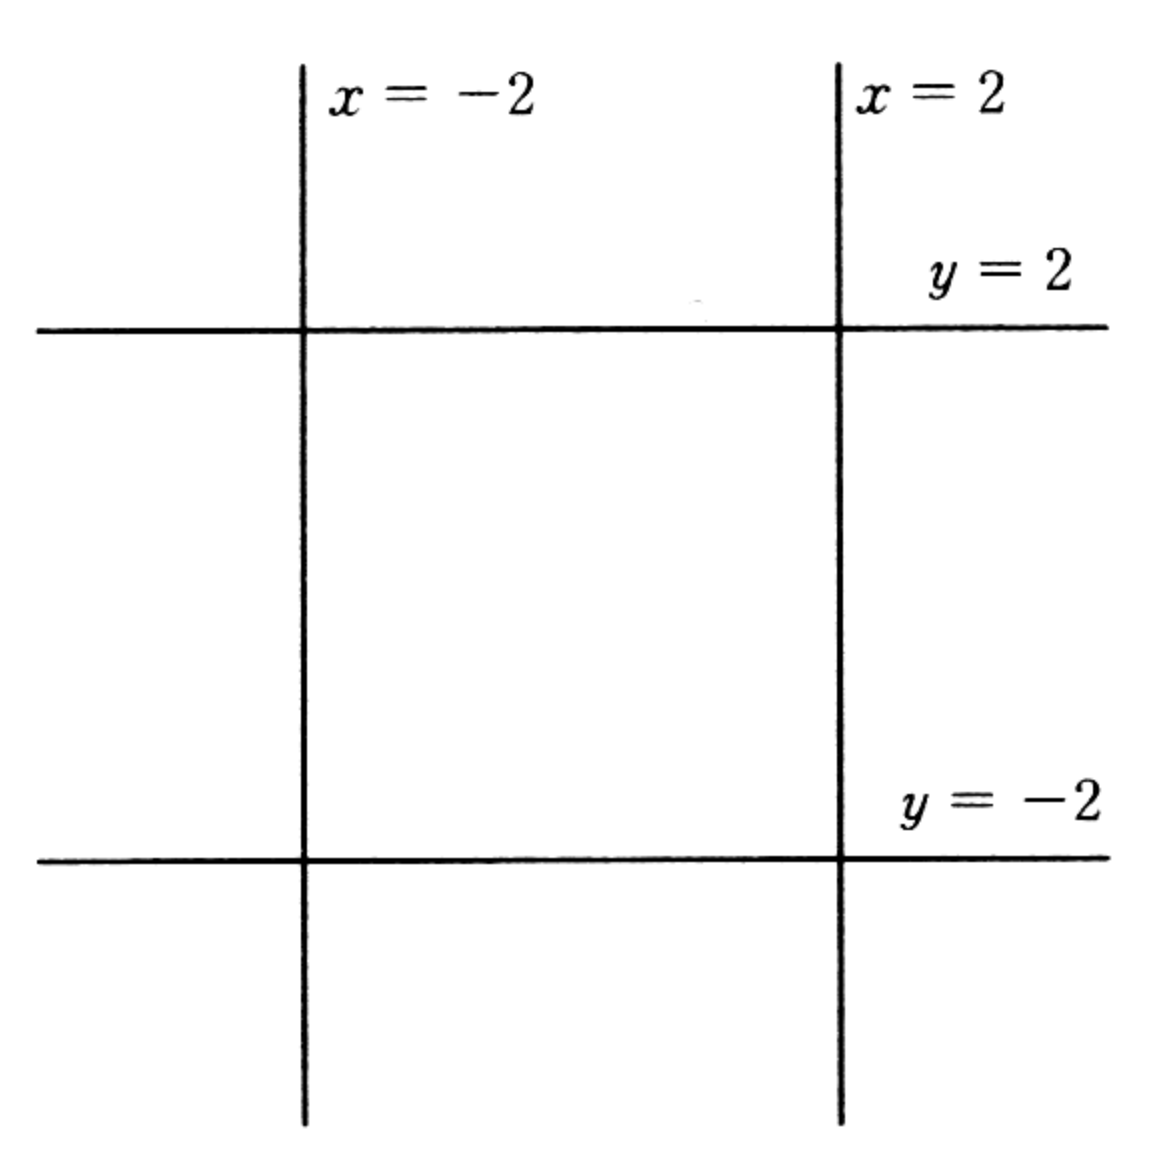
\includegraphics[width=0.42\linewidth]{figures/ch03-fig3.png}
  \figtitle{3}{零点集合（原书 p.44）}
\end{figure}
\begin{figure}[htbp]
  \centering
  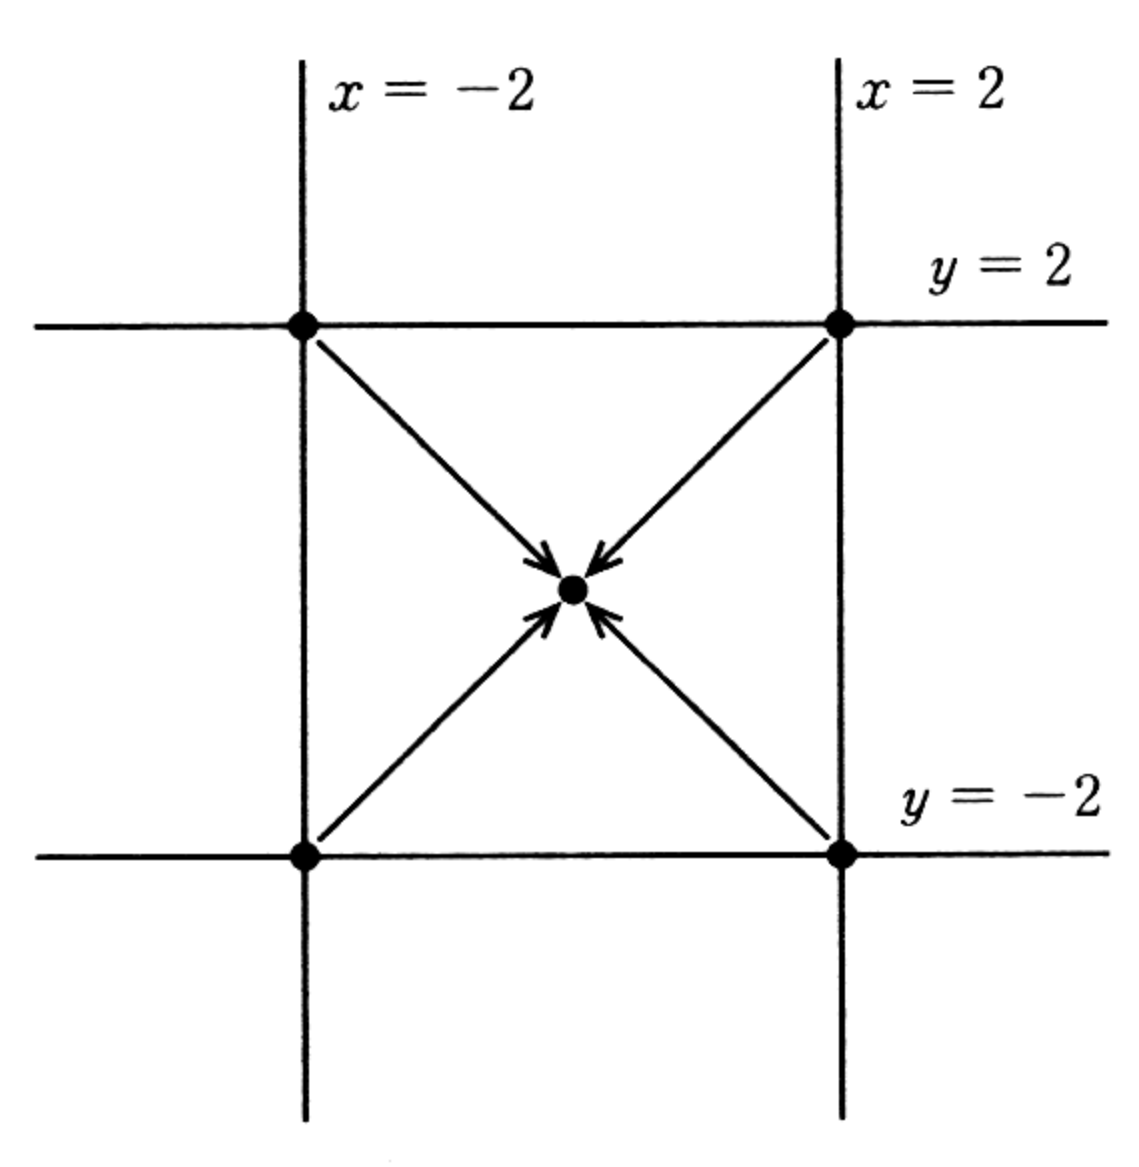
\includegraphics[width=0.50\linewidth]{figures/ch03-fig4.png}
  \figtitle{4}{$D_4$ 型的扩充 Dynkin 箭图（原书 p.44）}
\end{figure}%
接着考虑如图 5 那样的进一步变形，就得到 $D_4$ 型奇点 $-xy(x+y)$ 的变形\footnote{为简单起见，对 $x^3+xy^2$ 作了适当的变量替换。}
\[ -(x+2)(y+2)(x+y). \]
对它也套用上面的规则，就得到 $D_4$ 型的 Dynkin 箭图。把这里说明的内容准确写出来，就是同调镜像对称猜想
\begin{align}
  \mathcal{T}_{x^3+xy^2+z^2,\Z/6\Z} &\cong D^b\mathrm{Lag}(x^3+xy^2+z^2), \tag{10}\\
  D^b(\mathrm{coh}\,X_{2,2,2}) &\cong D^b\mathrm{Lag}(x^2+y^2+z^2-xyz) \tag{11}
\end{align}
的证明。对一般的 $(p,q,2)$，同调镜像对称猜想也几乎同样可以证明。

这里讲的“从画在实平面上的零点图读出消没闭链及其相交”的想法，是 A'Campo 在大约 30 年前引入的。当时恐怕没有人想到，它会成为连接奇点代数学与几何学的决定性钥匙。借助这把钥匙，正多面体群·轨道空间·奇点·（扩充）Dynkin 图之间那不可思议的关系（McKay 对应）得到了自然的说明，ADE 型奇点的同调镜像对称（范畴等价 (10) 与 (11)）也得以证明。通往新世界的大门就此打开。

\section{结语}

在本解说没有涉及的 $1/p+1/q+1/r<1$ 的世界里，有正多面体群
% ===== PDF p.053 (原书 p.45) =====
\begin{figure}[htbp]
  \centering
  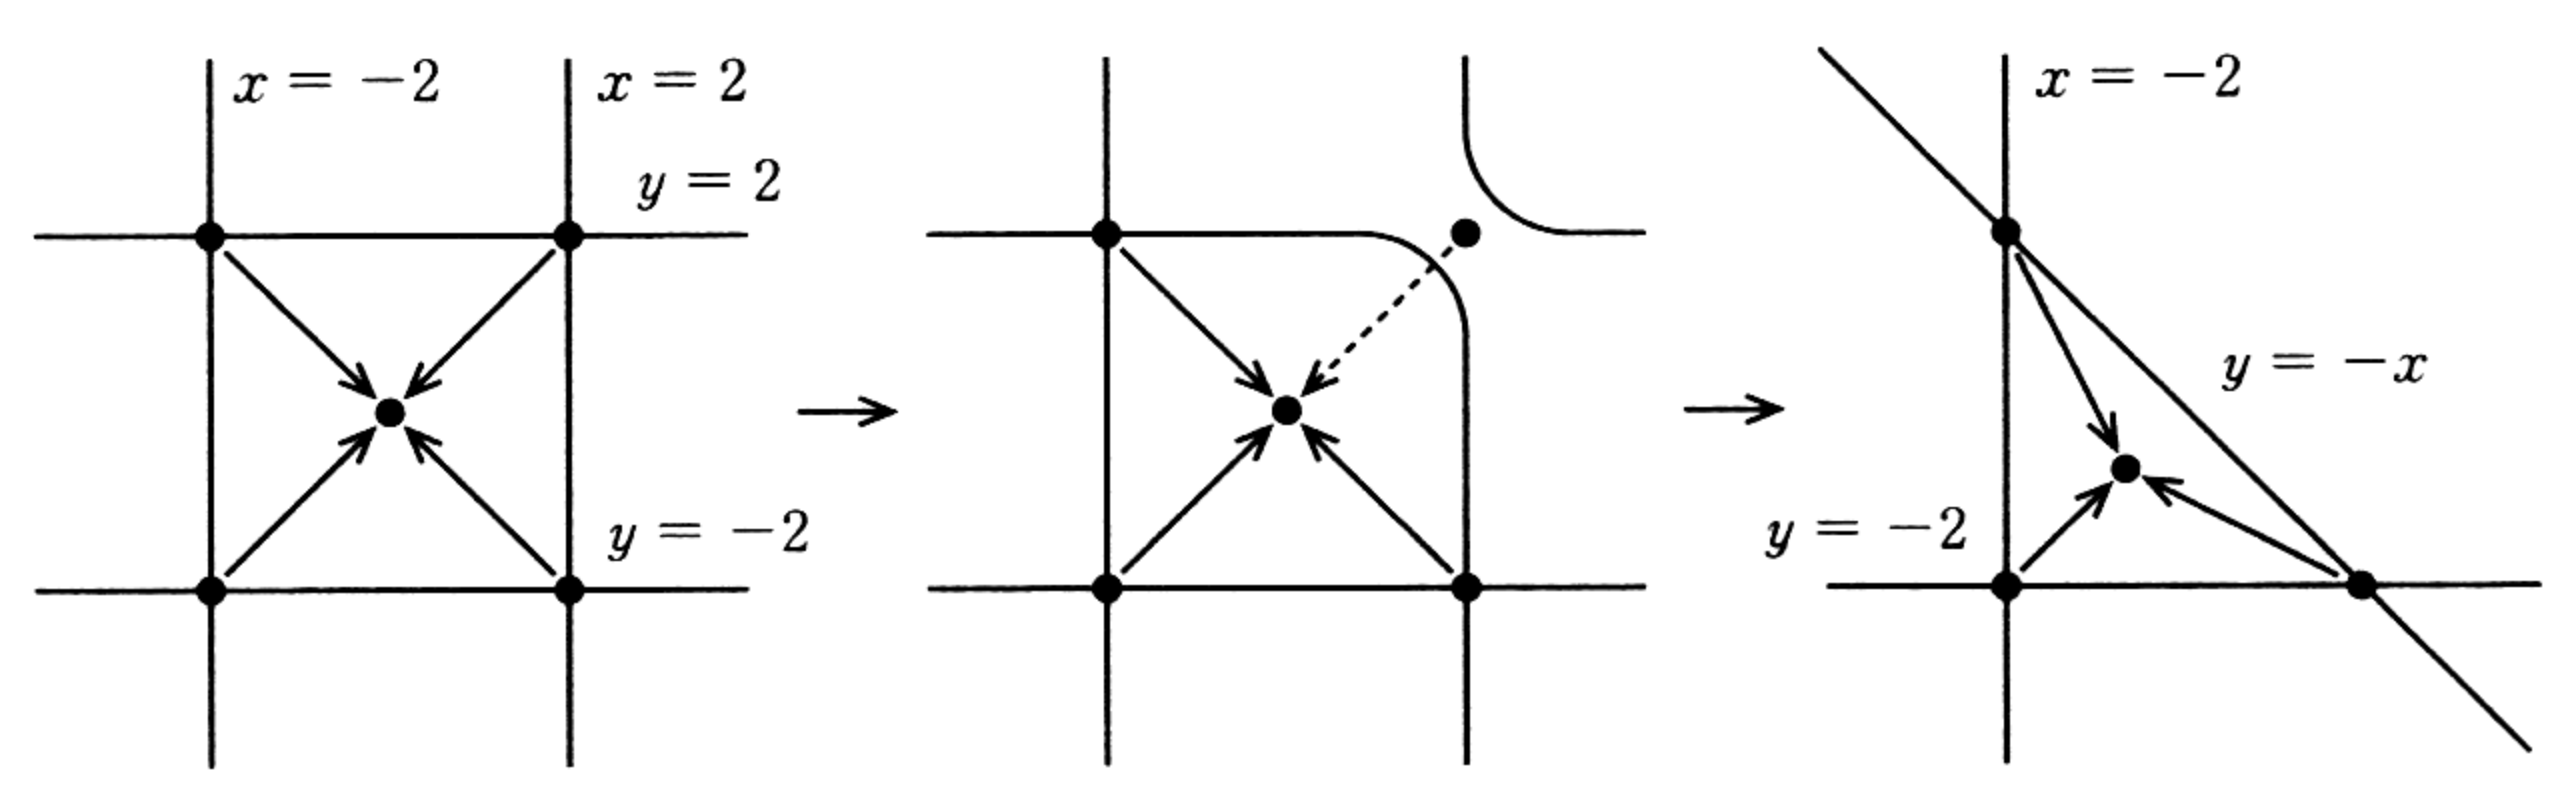
\includegraphics[width=0.95\linewidth]{figures/ch03-fig5.png}
  \figtitle{5}{从扩充 Dynkin 箭图到 Dynkin 箭图（原书 p.45）}
\end{figure}%
的推广——即 Schwarz 三角群理论——以及恰好位于 ADE 型奇点“背面”的 Arnold 例外型奇点等。这些领域里，有全貌尚未明朗、却非常有趣的数学。借助镜像对称以及在这一领域日新月异的研究手法，期待人们对它们的理解能取得飞跃性进展。

% 原书本章末无参考文献表（PDF p.053 即原书 p.45 为末页，只有图 5、末段与作者读音标记；PDF p.054 已是第 4 章章题页），故不设 reflist（reports/ch03.md 记一笔）。
% 原书章末作者读音标记［たかはし あつし］按 STYLE_GUIDE §3.7 省略不译，此处亦不留痕迹（reports/ch03.md 记一笔）。

% 本章原书节号用阿拉伯数字，正文中已用 \renewcommand{\thesection}{\arabic{section}}
% 切换；此处于章末显式恢复全书通用的罗马数字节号。
\renewcommand{\thesection}{\Roman{section}}

